%EDD uses a multi-objective fitness function with a FI2Pop genetic algorithm % for EDD, which accounts for two different but related objectives that are associated to the placement and distribution of elements, and the design patterns. The
%where fitness is %thus, 
%a weighted sum divided equally between (1) the inventorial aspect of the rooms, which relates to the placement of enemies and treasures in relation to doors and target ratios, and (2) the spatial distribution of the design patterns, which relates to the distribution between corridors and rooms, and the meso-patterns that those encompass. An in-depth explanation of EDD's fitness function can be found in~\citepthird{p3Alvarez2018a, Baldwin2017}.

%EDD uses a multi-objective fitness function with a FI2PoP genetic algorithm that optimizes (1) the inventorial aspect of the rooms, which relates to the placement of enemies and treasures in relation to doors and target ratios, and (2) the spatial distribution of the design patterns, which relates to the distribution between corridors and rooms, and the meso-patterns that those encompass. Both objectives are combined as a weighted sum divided equally.  An in-depth explanation of EDD's fitness function can be found in~\citepthird{p3Alvarez2018a, Baldwin2017}.

EDD uses a single-objective fitness function with a FI2Pop genetic algorithm where fitness is a weighted sum divided equally between (1) the inventorial aspect of the rooms, which relates to the placement of enemies and treasures in relation to doors and target ratios, and (2) the spatial distribution of the design patterns, which relates to the distribution between corridors and rooms, and the meso-patterns that those encompass. An in-depth explanation of EDD's fitness function can be found in~\citepthird{p3Alvarez2018a,p3Baldwin2017}.

%In addition, 
The overarching goal of MI-CC is to collaborate with the user to produce content, either to optimize (i.e. exploit) their current design towards some goal or to foster (i.e. explore) their creativity by surprising them with diverse proposals. By implementing MAP-Elites~\citepthird{p3Mouret2015} and continuous evolution into EDD, our algorithm can (1) account for the many dimensions that a user can be interested, (2) explore multiple areas of the search space and produce a diverse amount of high-quality suggestions to the user, and (3) still evaluate how interesting and useful the tile distribution is within a specific room. Henceforth, we name the presented approach \textbf{Interactive Constrained MAP-Elites} (IC MAP-Elites). 

\subsection{Illuminating Dungeon Populations with MAP-Elites}

MAP-Elites explores the search space more vastly by separating certain interesting dimensions, that affect different aspects of the room such as playability or visual aesthetics, from the fitness function, using them to categorize rooms into niches (cells). %as intrinsic measures of rooms to categorize them into niches (cells). %With such niches, we are able to present diverse suggestions to the user while still maintaining a high quality on them.

\subsubsection{Dimensions}

Dimensions in MAP-Elites are identified as those aspects of the individuals that can be calculated in the behavioral space, and that are independent of the fitness calculation. %intrinsic, and more important, independent from the fitness calculation. %, although, as we present in section \Cref{section:results}, the occurrence of individuals in certain dimensional cells correlates with lower or higher fitness scores. 
EDD offers the designer the possibility to choose among the following dimensions, two at a time:
%Currently, we use five different dimensions: (1) symmetry and (2) similarity, related to visual aesthetics, (3) number of meso-patterns and (4) spatial-patterns, related to the presence of patterns in the room, and used to exploit the design pattern characteristics of the room, and (5) linearity, linked to the type of gameplay and possibilities in the room. The user can only choose a pair of dimensions at a time, since presenting higher dimensions would be undesirable and non-understandable for the user. 

\textbf{Symmetry and Similarity.} We choose Symmetry as a consideration of the aesthetic aspects of the edited room since symmetric structures tend to be more visually pleasing. Similarity is used to present the user variations of their design but still preserving their aesthetical edits. Symmetry is evaluated along the X and Y axes, backslash and front slash diagonal and the highest value is used as to how symmetric a room is. Similarity is calculated through comparing tile by tile with the target room. Formulas, information and support for both evaluations are explained in greater details at~\citepthird{p3Alvarez2018a}, where both of them were used as aesthetic fitness evaluations.

\textbf{Number of Meso-patterns.} The number of meso-patterns correlates to the type and amount of encounters the designer wants the user to have in the room in a more ordered manner. The considered patterns are the treasure room (tr), guard rooms (gr), and ambushes (amb). Meso-patterns associate utility to a set of tiles in the room, for instance, a long chamber filled with enemies and treasures could be divided into 2 chambers, the first one with enemies and the second one with treasures so the risk-reward encounter is more understandable for the player. Since we already analyze the rooms for all possible patterns, the number of meso-patterns is simply $\#MesoPat=tr, gr, amb \in AllPatterns$. Equation (\ref{eq:meso-pat-eq}) presents the dimensional value, and since the used meso-patterns can only exist in a chamber, we normalize by the maximum amount of chambers in a room, which are of a minimum size of $3x3$, and results in $Max_{chambers}=\left\lfloor Cols/3 \right\rfloor * \left\lfloor Rows/3 \right\rfloor$.

%All variables will be defined, and such variables names will  be replaced

%\begin{equation} \label{eq:meso-pat-eq}
%D_{mesoPat} = \min{ \left\{     \dfrac{\#MesoPat}{Max_{chambers}}, 1.0}
%\right\} }
%\end{equation}

\begin{equation} \label{eq:meso-pat-eq}
D_{mesoPat} = \min \left\{ \dfrac{\#MesoPat}{Max_{chambers}}, 1.0 \right\}
\end{equation}


\textbf{Number of Spatial-patterns.} By spatial-patterns we mean chambers (c), corridors (cor), connectors (con), and nothing (n). We identify the number of spatial-pattern relates to how individual tiles group (or not) together to form spatial structures in the room. The higher the amount of spatial-patterns the lesser tiles will be group together in favor of more individualism. For instance, a room with one spatial-pattern can be one with no walls and just an open chamber, while a room with a higher number of spatial-patterns would subdivide the space with walls, using tiles for more specific patterns. Equation (\ref{eq:spatial-pat-eq}) presents how we calculate the value for such a dimension. The number of spatial patterns is simply $\#SpatialPat=c, n, cor, con \in AllPatterns$, we then normalize it by the largest side of the room and multiply it by a constant value, determined as $K=4.0$ through a process of experimentation since it resulted in a good estimation of the amount of spatial patterns in the room.

%\textit{not sure of this example} For instance, depicted in figure XXX a., a chamber is a micro-pattern that associate several tiles to one specific pattern, if we then simply add a wall in the middle of it as in figure XXX b., we break the pattern into many other patterns that in turn, create a different type of challenge for the user, a loop. We finally calculate the dimension value with the following formula:

%\begin{equation} 
%\label{eq:spatial-pat-eq}
%D_{spatialPat} = 
%\min{ \left\{ 
%    \frac{\#SpatialPat}{\max\left\{{Cols, Rows}\right\} * \textit{K}}, 1.0}
%\right\}
%\end{equation}

%\begin{equation} 
%\label{eq:spatial-pat-eq2}
%D_{spatialPat} = 
%\min{ \left\{ 
%    \frac{\#SpatialPat}{\max\left\{{Cols, Rows}\right\} * \textit{K}}, 1.0}\right\} }
%\end{equation}

\begin{equation} 
\label{eq:spatial-pat-eq}
D_{spatialPat} = \min\left\{\frac{\#SpatialPat}{\max\left\{{Cols, Rows}\right\} * \textit{K}}, 1.0\right\}
\end{equation}

\textbf{Linearity.} Linearity represents the number of paths that exist between the doors in the room. This relates to the type of gameplay the designer would like the room to have by the distributions of walls among the room. Having high linearity in a room does not need to only be by having a narrow corridor between doors but could also be generated by having all doors in the same open space (i.e. the user would not need to traverse other areas) or by simply disconnecting all paths between doors. Equation (\ref{eq:Linearity-eq}) shows the linearity calculation. Due to the use of patterns, we calculate the paths between doors as the number of paths that exist from a spatial-pattern containing a door to another. Finally, this is normalized by the number of spatial patterns in combination with the number of doors and their possible neighbors.

\begin{equation} \label{eq:Linearity-eq}
D_{lin} = 1 \text{--} \frac{AllPathsBetweenDoors} {\#spatialPat + \#NeighborsPerDoor}
\end{equation}

\subsubsection{Continuous Evolution}

%Creation tools are highly dynamic, the user might have an empty canvas in one moment, and after a few interactions over the course of some seconds, they might have a complex room with multiple paths and challenges for the user, and even more ideas on what to do next. Thus, the nature of the tool and the fast-paced interactions require a dynamic and continuous EA that can cope with the requirements of the user and adapt seamlessly to the new changes.

%This interesting paradigm shift, allows the user to focus solely in the design of the rooms while in the background, the EA is adapting to those new designs, rather than waiting for the EA to present suggestions.

EDD implements continuous evolution in two ways. First, the EA constantly updates the target room and configuration with the most recent version of the user’s design, and once the suggestions are broadcasted, that room is incorporated without changes to the population of individuals in the corresponding cell. Secondly, by changing the dimension information and their granularity for the MAP-Elites, which can be done at any given time by the designer. %&in which case, the EA recalculates the cells with the new dimensions and assign the population to the correct cell.% would reset all the cells, calculate their new dimension values and assign the previous populations to the correct cell.

Provided that EDD already uses a FI2Pop, we took as a starting point the constrained MAP-Elites presented by Khalifa et al.~\citepthird{p3Khalifa2018}, where the illuminating capabilities of MAP-Elites explore the search space with the constraints aspects of FI2Pop. This approach manages two different populations within each cell, a feasible and an infeasible one. Individuals move across cells when their dimension values change, or between the feasible and infeasible population according to their fulfillment of the feasibility constraint.

\algnewcommand\algorithmicforeach{\textbf{for each}}
\algdef{S}[FOR]{ForEach}[1]{\algorithmicforeach\ #1\ \algorithmicdo}

\algblockdefx{MRepeat}{EndRepeat}{\textbf{repeat}}{}
\algnotext{EndRepeat}

\begin{algorithm}
\caption{Interactive Constrained MAP-Elites}\label{alg:IC-MAPE}
\begin{algorithmic}[1]
\Procedure{IC-MAP-Elites($\protect[\{d_1,v_1\},...,\{d_n,v_n\}]$)}{}
\State $target \gets curEditRoom$ \Comment{Always in background}
\State createCells$(\protect[\{d_1,v_1\},...,\{d_n,v_n\}])$
\For{$i \gets 1$ to $PopSize$} %\Comment{$PopSize \gets 1000$}
     \State add mutate$(target)$ to $population$
\EndFor
\State CheckAndAssignToCell$(population)$ 
\While {true} \Comment{start continouous evo}
    \For{$generation \gets 1$ to $publishGen$}
        \If {$\textit{dimensionsChanged}$}
            \State $previousPop \gets cells_{pop}$
            \State createCells$(newDimensions)$
            \State checkAndAssignToCell$(previousPop)$ 
        \EndIf
        \MRepeat{ \text{[for feasible \& infeasible pop.]}}
            \For{$i \gets 1$ to $ParentIteration$}
                \State $curCell \gets \text{rndCell}(cells)$
                \State add tournament$(curCell)$ to $parent$
            \EndFor
            \State $offspring \gets  \text{crossover}(Parent)$
            \State checkAndAssignToCell$(offspring)$
        \EndRepeat
        \State sortAndTrim$(cells)$
    \EndFor
    \State broadcastElites() \Comment{render elites}
    \State $pop' \gets cells_{population}$
    \State add mutate$(cells_{pop})$ to $pop'$
    \State add $target$ to $pop'$
    \State checkAndAssignToCell $(pop')$
    \State sortAndTrim$(cells)$
\EndWhile
\EndProcedure
\Procedure{createCells(dimensions)}{}
    \ForEach{$dim \in dimensions $}
        \State add newCell$(dim_d, dim_v)$ to $cells$
    \EndFor
\EndProcedure
\Procedure{$\protect \text{check\&AssignToCell}(curPopulation)$}{}
    \ForEach{$individual \in curPopulation $}
        \State $individual_f \gets evaluate(individual)$ 
        \State $individual_d \gets dim(individual)$
        \State add $individual$ to $cell_{pop}(individual_d)$
    \EndFor
\EndProcedure
\end{algorithmic}
\end{algorithm}

\begin{figure*}[t]
\centerline{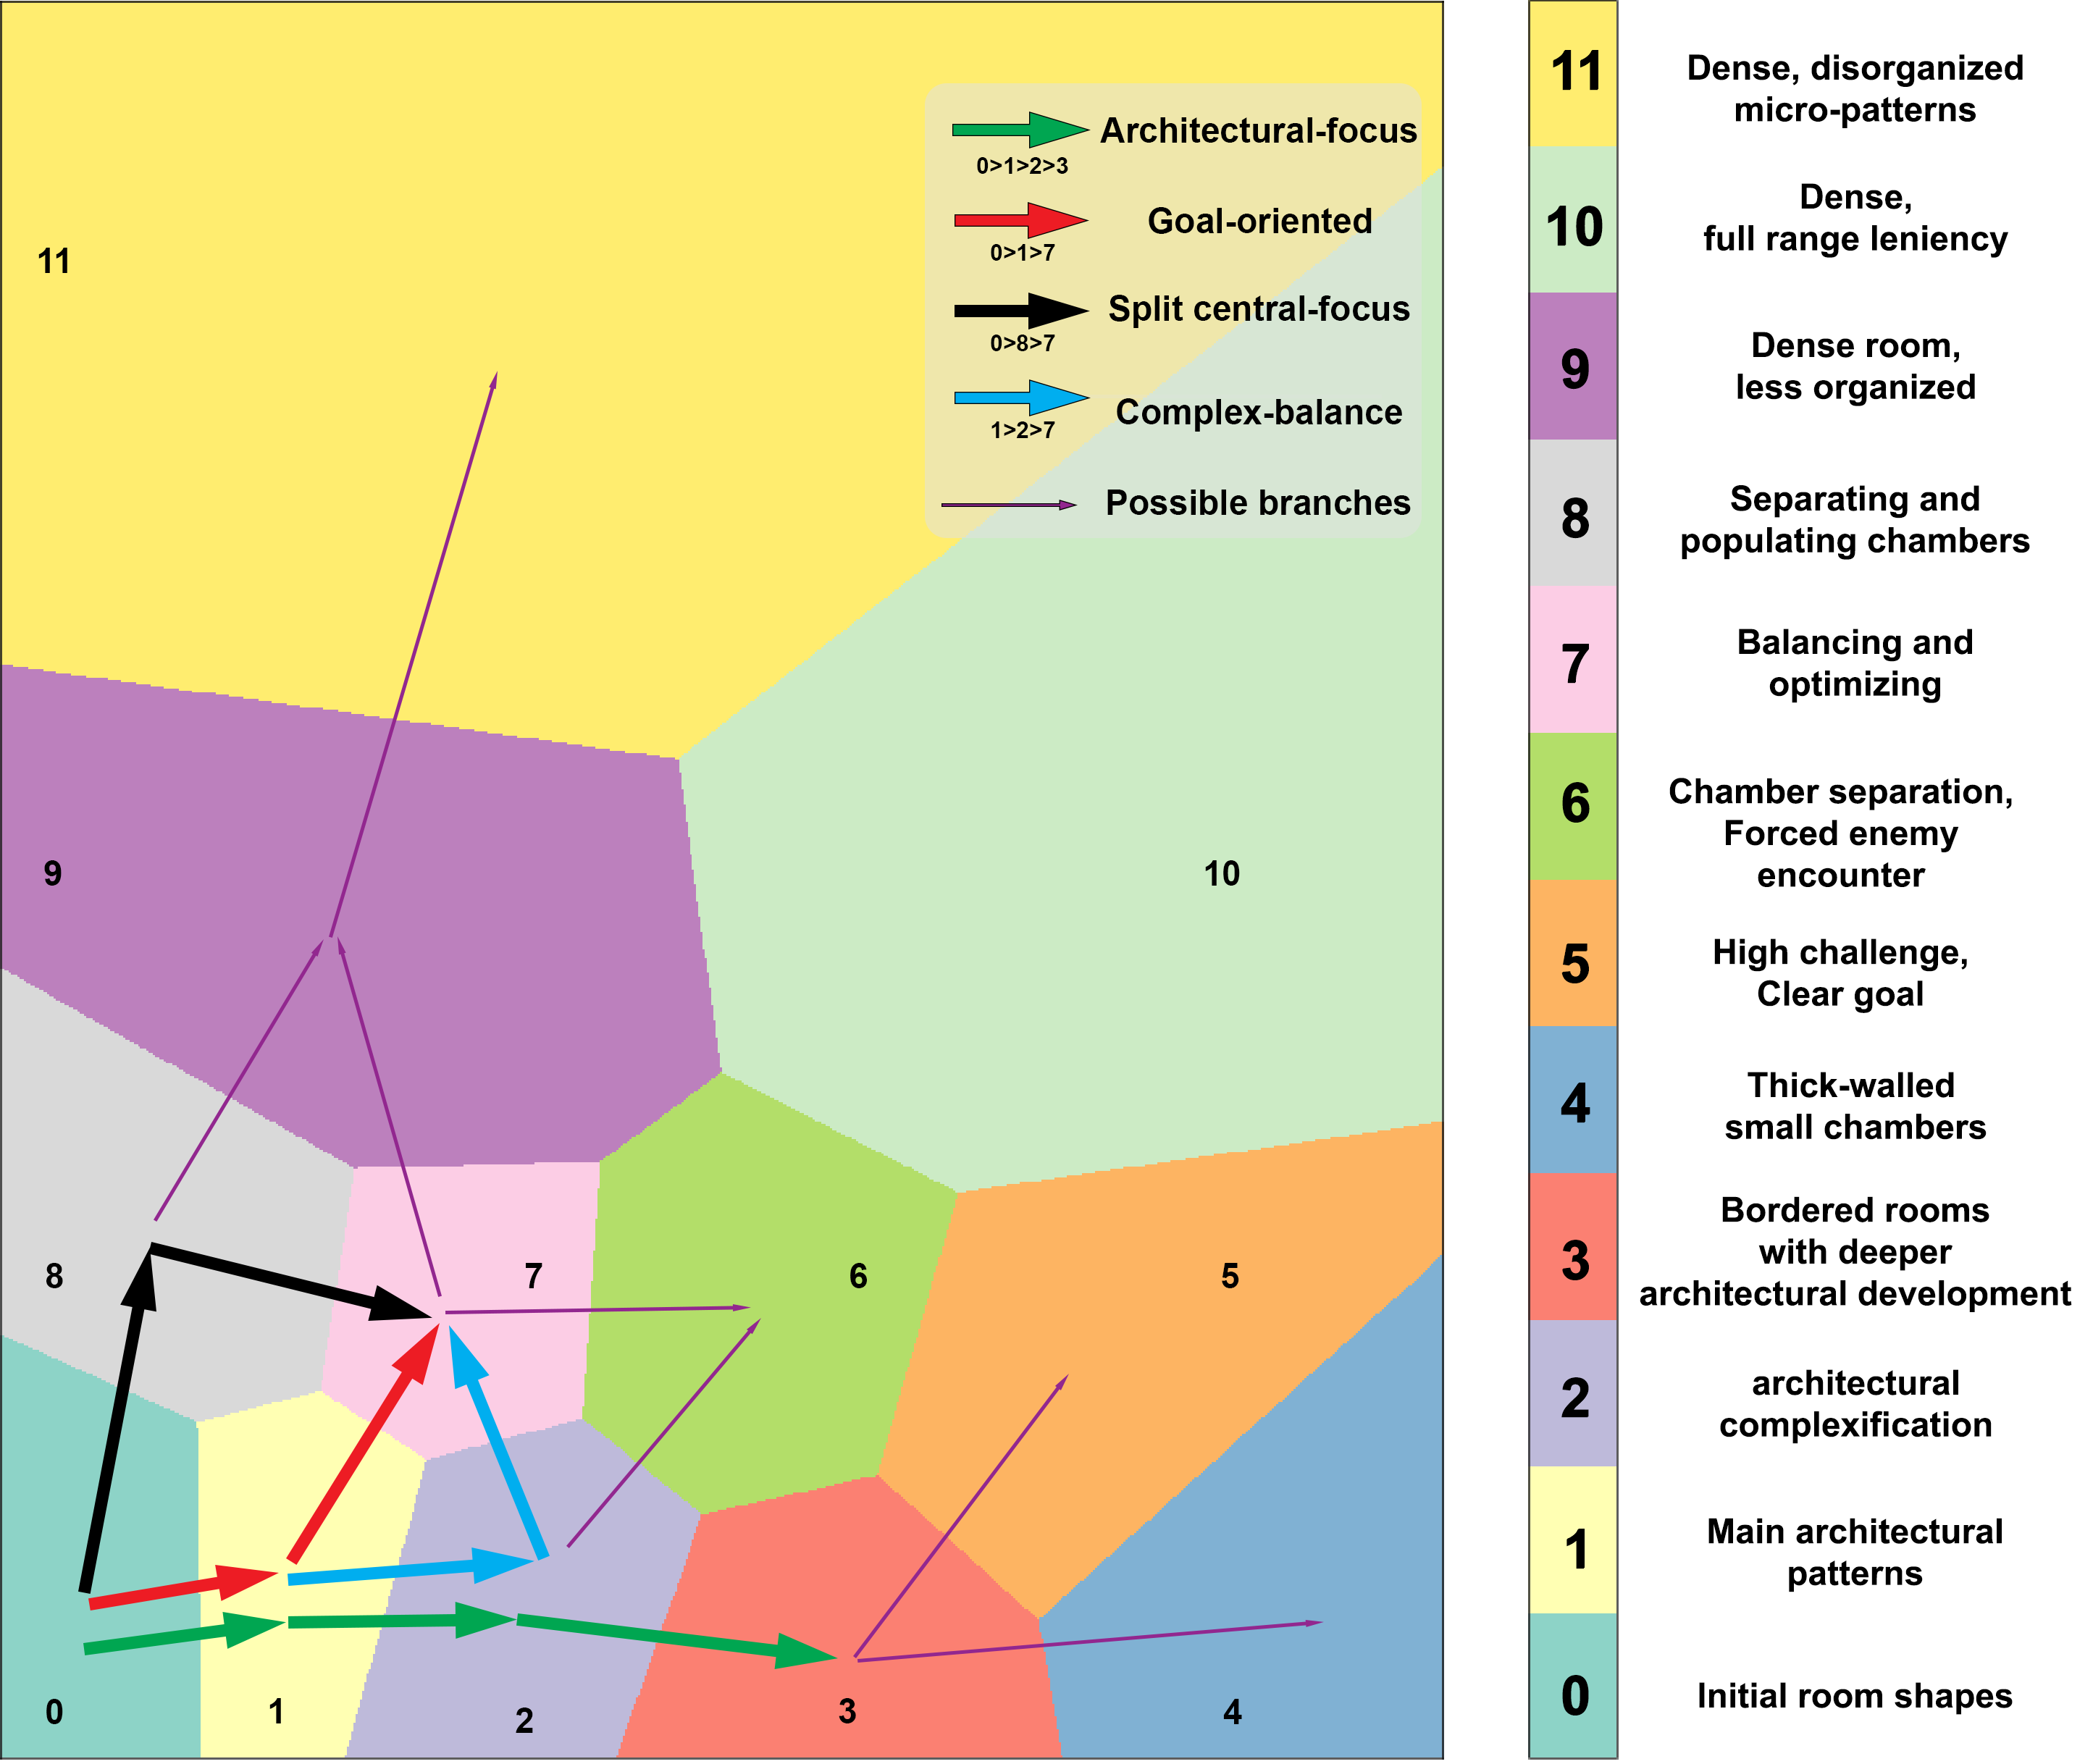
\includegraphics[width=18cm]{figure4.png}}
\caption{Rooms at generation $2090$ targeting Number of spatial-patterns (X) and Symmetry (Y). Each cell displays (top-right) the fitness of the optimal individual in its related feasible population. }
\label{figs:patt_sym}
\end{figure*}

\subsubsection{Algorithm}

The current evolutionary algorithm is depicted in Algorithm \ref{alg:IC-MAPE}. Cells are first created based on the dimensions selected by the user and proceed to initialize the population based on the user's design, evaluate it and assign each individual to the corresponding cell. Before starting each generation, we check if the dimensions have changed, and if so, recreate the cells and populate them with the previous individuals, and proceed through the evolutionary strategies. Selection is through tournament with a random number of competing parents and offspring are produced through a two-point uniform crossover with a chance of mutation. Offspring are placed in the correct cell and population after calculating their fitness and dimension's information. Finally, cells eliminate the low-performing individuals that over-cap their maximum capacity. Since interbreeding is not allowed, and can only happen indirectly (i.e. the offspring changing population and then used for breeding in consequent generations), the strategies are repeated for each of the population.

This procedure is repeated until the user decides to stop the algorithm. Meanwhile, the EA runs for $n$ generations, and once it reaches the specified limit, it broadcasts the found elites. In order to push the exploration, we first mutate all the individuals from all the populations and cells (while retaining the previous population), and add them into the same pool together with the current edited room without changes. Finally, we evaluate and assign all the individuals to the correct cells, and cells that are over maximum capacity eliminates low-performing individuals.

% Through suggestions based on their design, our EA provides an interesting proposal to the user evaluated with our multi-objective function, which was probably searched in the same exploration space niche as the rest of the population. However, there exist a vast amount of interesting rooms in the search space that are never explored, for instance, having narrow corridors between doors is not the only approach to get high linearity.

% to more interesting and diverse aspects for them. Increasing the granularity of a dimension correlates to the spreading of the already placed individuals into more specific \textbf{change word buckets} “buckets”, and reducing the granularity generalizes more the individuals in such a dimension. %would just mean a lost on expressiveness in order to have more general “buckets”.

% Although such a fitness works well to evaluate the composition of a room functionality-wise based on the design patterns, it falls short for considering all of the different forms of evaluations that a user can have over the provided suggestions.

% While it is crucial that the rooms within the dungeon are playable and feasible, it is not enough to account just for that, as users would like to permeate their rooms with different aesthetics, challenges, paths or even learning aspects. The design of a fitness function that can consider all these different factors and encompasses them into one single value is rather infeasible. The weighted sum of each factor takes away the importance to other aspects, and further aggregating several evaluation dimensions to the fitness function would thus, deepen such a problem.

%\begin{algorithmic}[1]
 % \State this is code \Comment{this is a comment}
%\end{algorithmic}

%\textit{[I think I should have a name for the process of check cell since I keep repeating it and it takes a considerably amount of space]}